\documentclass[twoside,openright,numbers,spanish]{ezthesis}
%% # Opciones disponibles para el documento #
%%
%% Las opciones con un (*) son las opciones predeterminadas.

%%
%% Formato de las referencias bibliogr'aficas:
%%   numbers          - numeradas, p.e. [1]
%%   authoryear (*)   - por autor y a'no, p.e. (Newton, 1997)
%%
%% Opciones adicionales:
%%   spanish         - tesis escrita en espa'nol
%%
%% Desactivar opciones especiales:
%%   nobibtoc   - no incluir la bibiolgraf'ia en el 'Indice general
%%   nofancyhdr - no incluir "fancyhdr" para producir los encabezados
%%   nocolors   - no incluir "xcolor" para producir ligas con colores
%%   nographicx - no incluir "graphicx" para insertar gr'aficos
%%   nonatbib   - no incluir "natbib" para administrar la bibliograf'ia

%% Paquetes adicionales requeridos se pueden agregar tambi'en aqu'i.
%% Por ejemplo:
%\usepackage{subfig}
%\usepackage{multirow}
\usepackage[spanish,activeacute]{babel}
\usepackage[utf8]{inputenc}
\usepackage{amsmath}
\usepackage{amsthm}
\usepackage{amssymb}
\usepackage{wrapfig}
\usepackage{minted}
\usemintedstyle{colorful}

%% # Datos del documento #
%% Nota que los acentos se deben escribir: \'a, \'e, \'i, etc.
%% La letra n con tilde es: \~n.

\author{Mar\'ia Fernanda Alcal\'a Durand}
\title{Aprendizaje Reforzado para el Juego de Distribuci\'on de Cerveza}
\degree{Maestra en Ciencia de Datos}
\supervisor{Dr. Adolfo Javier de Un\'anue Tiscare\~no}
\institution{Instituto Tecnol\'ogico Aut\'onomo de M\'exico}
\faculty{Divisi'on de Actuar\'ia, Estad\'istica y Matem\'aticas}
\department{Departamento Acad'emico de Matem\'aticas}

%% # M'argenes del documento #
%% 
%% Quitar el comentario en la siguiente linea para austar los m'argenes del
%% documento. Leer la documentaci'on de "geometry" para m'as informaci'on.

%\geometry{top=40mm,bottom=33mm,inner=40mm,outer=25mm}

%% El siguiente comando agrega ligas activas en el documento para las
%% referencias cruzadas y citas bibliogr'aficas. Tiene que ser *la 'ultima*
%% instrucci'on antes de \begin{document}.
\hyperlinking
\begin{document}

\graphicspath{{figs/}}

%% # Portada de la tesis #
%% ## Construye tu propia portada ##
%% 
%% Una portada se conforma por una secuencia de "Blocks" que incluyen
%% piezas individuales de informaci'on. Un "Block" puede incluir, por
%% ejemplo, el t'itulo del documento, una im'agen (logotipo de la universidad),
%% el nombre del autor, nombre del supervisor, u cualquier otra pieza de
%% informaci'on.
%%
%% Cada "Block" aparece centrado horizontalmente en la p'agina y,
%% verticalmente, todos los "Blocks" se distruyen de manera uniforme 
%% a lo largo de p'agina.
%%
%% Nota tambi'en que, dentro de un mismo "Block" se pueden cortar
%% lineas usando el comando \\
%%
%% El tama'no del texto dentro de un "Block" se puede modificar usando uno de
%% los comandos:
%%   \small      \LARGE
%%   \large      \huge
%%   \Large      \Huge
%%
%% Y el tipo de letra se puede modificar usando:
%%   \bfseries - negritas
%%   \itshape  - it'alicas
%%   \scshape  - small caps
%%   \slshape  - slanted
%%   \sffamily - sans serif
%%
%% Para producir plantillas generales, la informaci'on que ha sido inclu'ida
%% en el archivo principal "tesis.tex" se puede accesar aqu'i usando:
%%   \insertauthor
%%   \inserttitle
%%   \insertsupervisor
%%   \insertinstitution
%%   \insertdegree
%%   \insertfaculty
%%   \insertdepartment
%%   \insertsubmitdate
%\maketitle

\begin{titlepage}
\begin{center}
\Large {INSTITUTO TECNOLÓGICO AUTÓNOMO DE MÉXICO}

 \vspace{0.5 cm}
  \centering
    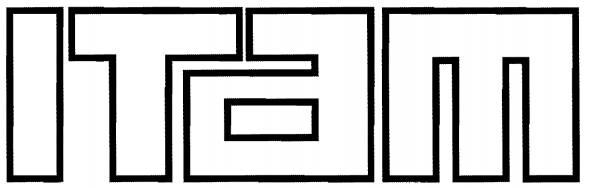
\includegraphics[scale=0.5]{logoITAM.jpg}

 \vspace{0.5 cm}
 \textbf{Aprendizaje Reforzado para el Juego de la Distribuci\'on de Cerveza}
  \vspace{2 cm}\\
  \Huge{\textbf{T \ \ \ \ \ \ E \ \ \ \ \ S \ \ \ \ \ I \ \ \ \ \ \ S}}
    \vspace{.4cm}\\
  \Large{QUE  \ \ PARA \ \ \ OBTENER \ \ \ EL \ \ \ TÍTULO \ \ DE 
   \vspace{.4cm}\\
  MAESTRA EN CIENCIA DE DATOS 
   \vspace{.4cm}\\
  P \ \ \ \ \ \ \ R \ \ \ \ \ \ E \ \ \ \ \ \ S \ \ \ \ \ \ E \ \ \ \ \ \ N \ \ \ \ \ \ T \ \ \ \ \ \ \ A 
   \vspace{.4cm}\\
 \textbf{MAR\'IA \ \ FERNANDA\ \ ALCAL\'A \ \ DURAND}}
    \vspace{1 cm}\\
\normalsize \textbf{ASESOR: DR. ADOLFO JAVIER DE UN\'ANUE TISCARE\~NO}
\vspace{1cm}\\
MÉXICO, D.F \hfill{2016}
\end{center}
\end{titlepage}

%% Nota 1:
%% Se puede agregar un escudo o logotipo en un "Block" como:
%%   \TitleBlock{\includegraphics[height=4cm]{escudo_uni}}
%% y teniendo un archivo "escudo_uni.pdf", "escudo_uni.png" o "escudo_uni.jpg"
%% en alg'un lugar donde LaTeX lo pueda encontrar.

%% Nota 2:
%% Normalmente, el espacio entre "Blocks" se extiende de modo que el
%% contenido se reparte uniformemente sobre toda la p'agina. Este
%% comportamiento se puede modificar para mantener fijo, por ejemplo, el
%% espacio entre un par de "Blocks". Escribiendo:
%%   \TitleBlock{Bloque 1}
%%   \TitleBlock[\bigskip]{Bloque2}
%% se deja un espacio "grande" y de tama~no fijo entre el bloque 1 y 2.
%% Adem'as de \bigskip est'an tambi'en \smallskip y \medskip. Si necesitas
%% aun m'as control puedes usar tambi'en, por ejemplo, \vspace*{2cm}.




%% # Prefacios #
\preface
%% Las secciones del "prefacio" inician con el comando \prefacesection{T'itulo}
%% Este tipo de secciones *no* van numeradas, pero s'i aparecen en el 'indice.
%%
%% Si quieres agregar una secci'on que no vaya n'umerada y que *tampoco*
%% aparezca en el 'indice, usa entonces el comando \chapter*{T'itulo}
%%

\newpage
\mbox{}
\thispagestyle{empty} % para que no se numere esta página

\newpage
\thispagestyle{empty}
Con fundamento en los art'iculos 21 y 27 de la Ley Federal del
Derecho de Autor y como titular de los derechos moral y patrimonial de la obra titulada ``\textbf{Aprendizaje Reforzado para el Juego de Distribuci\'on de Cerveza}'', otorgo de manera gratuita y permanente al Instituto Tecnol'ogico Aut'onomo de M'exico y a la Biblioteca Ra'ul Baill\`eres Jr., autorizaci'on para que fijen la obra en cualquier medio, incluido el electr'onico, y la divulguen entre sus usuarios, profesores, estudiantes o terceras personas, sin que pueda percibir por tal divulgación una contraprestación.

\vspace{20 mm}
\begin{center}
Mar'ia Fernanda Alcal'a Durand\\

\vspace{20 mm}
\makebox[2in]{\hrulefill}\\
FECHA\\
\vspace{20 mm}
\makebox[2in]{\hrulefill}\\
FIRMA
\end{center}

\newpage
\mbox{}
\thispagestyle{empty} % para que no se numere esta página


\prefacesection{Agradecimientos}

En este momento, le agradezco a Drake por hacer m\'usica tan espantosamente repetitiva: mi cerebro lo toma como ruido blanco y puedo concentrarme muy bien.

\newpage
\mbox{}
\thispagestyle{empty} % para que no se numere esta página


%% # 'Indices y listas de contenido #
%% Quitar los comentarios en las lineas siguientes para obtener listas de
%% figuras y cuadros/tablas.
\tableofcontents
%\listoffigures
%\listoftables

%% # Cap'itulos #
\cuerpo
\chapter{Introducci'on}

\textit{Necesito una cita cool para empezar mi tesis.}
\begin{flushright}
 Fleo
 \end{flushright}

\vspace{10 pt}


%business dynamics
%sistemas complejos adaptativos
%poner ejemplos?

%dynamic stability : edge of chaos. no es que sean caóticos sino que la mayor parte de las fluctuaciones pequeñas se las comen los feedback, pero la línea de qué es "pequeño" no es nada clara
%ley de Ashby: para poder controlar algo, se necesita al menos igual nivel de complejidad


Uno de las principales dificultades de las cadenas de suministro es que los agentes encargados de optimizar las estrategias solamente pueden tomar decisiones "dentro" del eslabón en el que se encuentran, y no tienen información más allá de los eslabones inmediatemente conectados. Así, la información acerca de la demanda del consumidor se va diluyendo en cada nivel, además de que las decisiones tomadas tienen repercusiones más allá del futuro inmediato. \\

Los agentes optimizadores deben tratar de inferir el patrón global por medio de información local bastante restringida. Sin embargo, los datos que reciben obedecen al tiempo real y no tienen la oportunidad de repetir experimentos.\\

Un modelo computacional que se comporte suficientemente parecido al mundo real, en el que todos los demás eslabones tomen estrategias que también maximizarían sus beneficios podría dar una opción: el experimento es replicable tantas veces como sea necesario y cada eslabón puede conocer una extrategia óptima para una gran cantidad de demandas de consumidor posibles.\\

En este trabajo se modelará el Problema de Distribución de Cerveza, \textit{The Beer Distribution Game}, planteado por primera vez en la Escuela de Administraci\'on y Direcci\'on de Empresas Sloan del MIT en los años 60\footnote{En este momento no cuento con la fuente original.}, \\

Este documento tiene un formato simple y una estructura de propuesta de proyecto a propósito, dado que se pretende continuar trabajando en este proyecto hasta concretar una Tesis para obtener el grado de Maestría en Ciencia de Datos.
\section{Reinforcement Learning: conceptos}

Su principio se basa en la psicolog\'ia conductista: un \textit{agente} busca ser recompensado por un premio, el cual obtiene cuando realiza una secuencia de \textit{acciones} que lo llevan a concluir una tarea exitosamente. Adem\'as, para maximizar la cantidad de \textit{recompensa} que recibe - o, alternativamente, minimizar el tiempo que espera entre un premio y el siguiente - comienza a optimizar su pol\'itica (\textit{$\pi$}) para llegar a la meta satisfactoriamente.\\

La principal caracter\'istica del agente es que tiene la capacidad de tomar decisiones sobre sus acciones, las cuales son su forma de interactuar con el \textit{mundo}, llev\'andolo de un \textit{estado} a otro. El agente no tiene acceso a todas las consecuencias de sus acciones; de hecho, ni siquiera conoce todo el mundo.\\

El agente toma una acci\'on en el tiempo $t$, la cual depende del estado $s_t$ del mundo. En $t+1$, el mundo reaccion\'o ya a la interacci\'on del agente con \'el, as\'i que el agente recibe una recompensa $r_{t+1}$ y toma una nueva acci\'on dependiendo del estado $s_{t+1}$ del mundo. Sin embargo, no es \'optimo seleccionar acciones solamente con base en la recompensa $r_{t+1}$, pues la naturaleza temporal del problema lo convierte en un problema a largo plazo, y el agente estar\'ia considerando solamente consecuencias en el corto plazo.\\

As\'i, el agente debe aprender que existe un \textit{retraso} entre cada acci\'on que toma y el premio. Supongamos que, en una cuadr\'icula, el premio se encuentra en la casilla (x,y). El agente solamente puede llegar a esa casilla meta desde las adyacentes, pero si no se encuentra en una de estas, primero debe acerc\'arseles. As\'i, cuando el agente comienza su exploraci\'on, ir\'a aprendiendo que, lejos de que la recompensa sea inmediata, debe tomar una secuencia de acciones para llegar a ella.\\

Podemos entonces definir la \textit{funci\'on de valor} asociada a la pol\'itica como el valor esperado de la recompensa al tiempo $t$ dado que el agente se encuentra en el estado $s$.\\



%Esta recursi\'on es conocida como \textit{Ecuaci\'on de Bellman}.

Tambi\'en es necesario que el agente ajuste su comportamiento mientras transcurre el tiempo: al principio debe explorar para conocer la mayor cantidad de consecuencias a sus acciones posibles, pero debe mantener el conicimiento de cu\'ales acciones le han reportado buenas acciones y tomar esas decisiones m\'as seguido. A esta estrategia de exploraci\'on se le llama $\epsilon-greedy$.\\

Definamos $p_r{t}$ y $p_t{t}$ como las probabilidades al tiempo $t$ de exploraci\'on y explotaci\'on, respectivamente. Entonces:

\vspace{-30pt}
\begin{align*}
p_r{t} &= 1 - \epsilon(t) \\
p_t{t} &= 1 - p_r{t} \quad \quad \forall t
\end{align*}

La funci\'on $\epsilon$ suele ser implementada como decreciente de forma lineal para el aprendizaje, de tal forma que mientras pasa el tiempo, el agente escoge las acciones conocidas que le reportan mayor utilidad m\'as seguido; junto con un par\'ametro $\ro$ aleatorio para asegurar que siempre existe una probabilidad positiva de explorar.\\

Generalmente se supone este tipo de problemas como Procesos de Decisi\'on de Markov (MDP), cuya principal caracter\'istica es que cumplen con la famosa propiedad de Markov: a grandes rasgos, el futuro solamente depende del presente, no del pasado.\\

%queremos aprender la funci\'on de valor

Cuando la pol\'itica a tomar es dif\'icil de aprender porque no tenemos ejemplos, o el mundo / conjunto de acciones / conjunto de consecuencias es demasiado grande, es apropiado utilizar Aprendizaje Reforzado en lugar de Aprendizaje de M\'aquina regular.

\section{Aprendizaje Reforzado}

\subsection{Q-Learning: conceptos}

%empezar con Q propuestas: generalmente 0 o -inf, e ir arreglando conforme vamos encontrando caminos a la meta

%hay que revisitar

%aqui se pone la definicion de Q
$$
V(s) = \max_{a}{Q(s,a)}
$$
$$
Q(s, a) = R(s, a) + \gamma * \max_{a}{Q(s^{'}, a^{*})}
$$

Donde $s{'}$ es el siguiente estado, y $a^{*}$ representa todas las acciones posibles. Al estimar la funci\'on $Q$ para cada par de estado con acci\'on, es posible encontrar la mejor acci\'on para cada estado y, as\'i, obtener una pol\'itica \'optima.

\subsubsection{Algoritmo}

\begin{enumerate}
    \item Asignar $Q(s,a) = 0$ para todos los estados y acciones.
    \item Posicionarse en un estado $s$
    \item Seleccionar acci\'on $a^{*}$ y ejecutar
    \item Recibir recompensa $r$
    \item Observar estado nuevo $s^{'}$
    \item Actualizar $\hat{Q}(s,a) = r(s,a) + \lambda \max _{ a^{'} }{  \hat{Q}(s^{'},a^{'}) }$
    \item Asignar nuevo estado $s \leftarrow s^{'}$
    \item Volver a 2 hasta convergencia
\end{enumerate}



\section{Modelo Multiagente}

%Los agentes no se comunican
%Alguna cosa de system dynamics
%Considera consecuencias globales de interacciones locales
% Rules regulate the behaviour of the system by specifying local relationships and transitions between states

%Causal loop diagrams emphasize he feedback structure of the system
% stock and flow diagrams emphasize the underlying physical structure. must be causal, no correlations!
%indicate important delays

En este trabajo, consideraremos a cada eslab\'on de la cadena de suministro como un agente. 

\begin{minted}
[
frame=leftline,
framesep=2mm,
baselinestretch=1.2,
fontsize=\footnotesize,
linenos
]
{python}
class State(agent)
	def __init__(self,inventory):
		self.inventory = inventory
		self.upstream
		self.downstream
		self.backlog

	def receive_upstream(self,orders):
		self.upstream = orders

	def give_downstream(self,orders):
		self.downstream = orders

	def update_inventory(self,orders_in,orders_out):
		self.inventory = self.inventory + orders_in - orders_out
		
	def backlog_penalty(self,orders):
		self.backlog = orders*penalty_fee

\end{minted}
Con las siguientes definiciones:

\begin{minted}
[
frame=leftline,
framesep=2mm,
baselinestretch=1.2,
fontsize=\footnotesize,
linenos
]
{python}

# Agent variables

agent.inventory[t]  #what the agent has on the warehouse
agent.upstream[t]   #upstream orders.
                    #fulfilled immediately but constrained to have enough
agent.downstream[t] #downstream orders
agent.backlog[t]    #backlogged orders

# Global variables

beer_price          #cost per product unit
warehouse_cost      #holding in warehouse per time unit per product unit
penalty_fee         #backlog orders cost. 
                    #not fulfilling orders leave clients unhappy
\end{minted}

Cada agente solamente puede comunicarse con los niveles inmediatamente vecinos; es decir, las \'unicas interacciones que puede tener con el mundo son el n\'umero de \'ordenes que recibe del nivel inferior y el inventario que pide al nivel superior. Sin embargo, como hemos definido una penalizaci\'on por mantener cerveza en el inventario (el costo del almac\'en), la decisi\'on concerniente a la petici\'on del nivel inferior queda determinada: vender\'a todo lo que pueda, pues cada venta le reporta una ganancia, y no llenar la orden completa cuando tiene suficiente inventario lo har\'ia incurrir en un costo innecesario.\\

Esto quiere decir que, para cada agente, el conjunto de \textbf{acciones} que puede tomar es solamente el n\'umero de cervezas que pedir\'a al nivel inmediatamente superior en cada tiempo $t$. Esta acci\'on est\'a declarada por:

\begin{minted}
[
frame=leftline,
framesep=2mm,
baselinestretch=1.2,
fontsize=\footnotesize,
linenos
]
{python}
agent.upstream[t]
\end{minted}

Por lo tanto, lo que tendr\'a guardado en la bodega en el tiempo $t$ estar\'a constituido por el n\'umero de cervezas que ten\'ia en el tiempo anterior $t-1$, menos el n\'umero de cervezas vendidas, m\'as el n\'umero de cervezas que recibe del nivel inmediatamente superior por el pedido de reaprovisionamiento.\footnote{Se agregan algunas indentaciones y saltos de l\'inea al c\'odigo para facilitar claridad de lectura.}\\

\begin{minted}
[
frame=leftline,
framesep=2mm,
baselinestretch=1.2,
fontsize=\footnotesize,
linenos
]
{python}
agent.inventory[t] =    agent.inventory[t-1] + \
                        agent.upstream[t] - agent.downstream[t]
\end{minted}

Restringido a que cada agente solamente cubrir\'a la orden del nivel inferior si tiene suficiente inventario para hacerlo (es por esto que en la definici\'on de clase no se utilizan las variables expl\'icitas, sino $orders\_in$ y $orders\_out$.\\

Su recompensa est\'a dada por:

\begin{minted}
[
frame=leftline,
framesep=2mm,
baselinestretch=1.2,
fontsize=\footnotesize,
linenos
]
{python}

agent.reward[t] =   beer_cost * agent.downstream[t] - \
                    warehouse_cost * agent.inventory[t] - 
                    penalty_fee * agent.backlog[t]
\end{minted}

El objetivo de cada agente es maximizar su recompensa. Sin embargo, este es un problema ligeramente diferente a los comunes de \textit{Q-learning}, en los cuales el valor de la recompensa es conocido y, una vez encontrado, se buscan las acciones \'optimas ``de atr\'as hacia adelante'' (como el ejemplo t\'ipico de una cuadr\'icula).\\

%%%%%%%%%%%%%%%%%%%%%%%%%%%%%%%%%%%%%%
%%%%%%%%%%%%%%%%%%%%%%%%%%%%%%%%%%%%%%
%%%%%%%%%%%%%%%%%%%%%%%%%%%%%%%%%%%%%%
%%%%%%%%%%%%%%%%%%%%%%%%%%%%%%%%%%%%%%
%%%%%%%%%%%%%%%%%%%%%%%%%%%%%%%%%%%%%%

Su pol\'itica est\'a definida con base en la funci\'on Q, una vez que el proceso de aprendizaje fue finalizado, de esta manera, puede realizar una b\'usqueda sobre todas las posibles acciones en los estados y sencillamente escoger la mejor, lo cual converge a la pol\'itica (cuasi)\'optima. Tal pol\'itica se puede definir como:

\begin{minted}
[
frame=leftline,
framesep=2mm,
baselinestretch=1.2,
fontsize=\footnotesize,
linenos
]
{python}
Pi(s) = [retailer.upstream[s],wholesaler.upstream[s],\
        distributor.upstream[s],manufacturer.upstream[t]]
\end{minted}

Es importante destacar que este sistema toma solamente una de las ramas que existen en la industria de cualquier producto (existe m\'as de un minorista, etc.), e incluso, toma solamente un producto. A\'un as\'i, es un sistema complejo bastante robusto y sensible a cambios peque\~nos.
\chapter{El Problema: Juego de Distribuci\'on de la Cerveza}

%The purpose of the game is to understand the distribution side dynamics of a multi-echelon supply chain used to distribute a single item, in this case, cases of beer.


%There is a one-point cost for holding excess inventory and a one-point cost for any backlog (old backlog + orders - current inventory).

%The game is used to illustrate one of the links between System Dynamics theory and the Feedback Control Theory which inspired it - that systems with positive feedback loops and high gain can lead to oscillation and overload,

La estructura se puede observar en la figura \ref{diagram_wikipedia}.\footnote{Imagen tomada de la página de Wikipedia \textit{The Beer Distribution Game}, bajo la licencia Creative Commons Attribution-Share Alike 3.0 Unported}\\


\begin{figure}[h]
\caption{Distribución de Cerveza}
\label{diagram_wikipedia}
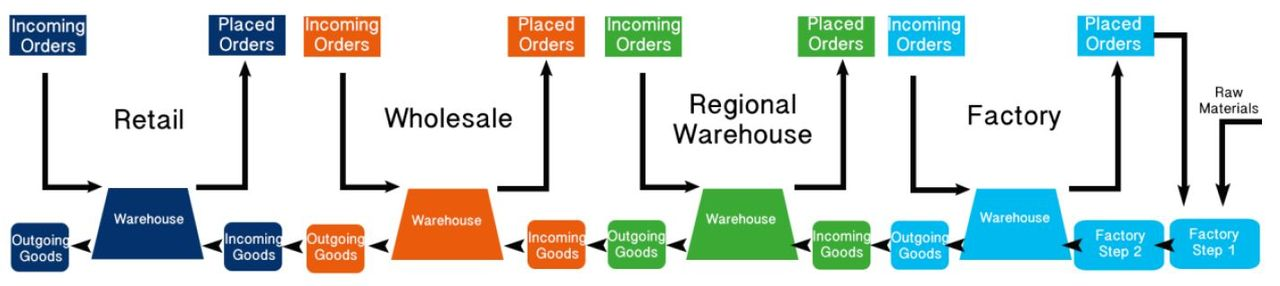
\includegraphics[width=8cm]{Diagrama_Wikipedia.JPG}
\centering
\end{figure}

Las variables que tienen efecto en este problema son:
\begin{itemize}
    \item Demanda del Consumidor
    \item Tiempo de Ajuste de Inventario
    \item Tiempo de Envío
    \item Tiempo de Producción
\end{itemize}

Para cada uno de los agentes: tiendas minorista, mayorista y de distribución, y fábrica.\\

Este problema se ha estudiado antes por \citet{Strozzi}, por medio de Algoritmos Genéticos y por \citet{Chaharsooghi} por medio de $Q-learning$. Ambas metodolog\'ias \\

El aporte de este trabajo será agregar un componente de estacionalidad en el proveedor de la fábrica: el campo.

\subsection{\textit{Efecto Látigo}}

El \textit{Efecto Látigo} se ejemplifica con el siguiente escenario:


\begin{enumerate}
    \item El comprador, que generalmente compra $6$ cervezas, ahora quiere $10$, pero la tienda minorista solamente cuenta con $7$. El minorista le venderá todo su inventario, pues es la acci\'on que maximiza su ganancia. Debe decidir si volverá a tener un inventario de $6$ o si debe pedir un número mayor de cervezas, atendiendo la aparentemente creciente demanda. Decide pedir $9$ cervezas al siguiente nivel, la tienda de mayoreo.
    \item El mayorista cuenta con $17$ cervezas. Llena el pedido del minorista, pero decide que ten\'ia guardado demasiado inventario, as\'i que se queda con $8$ cervezas en su almac\'en, sin hacer una orden al siguiente nivel, la tienda de distribución.
    \item La tienda de distribuci\'on decide comprar $1$ unidad
\end{enumerate}

En este escenario, el mayorista obtuvo informaci\'on distorsionada acerca del repentino crecimiento en la demanda del comprador, mientras que la tienda de distribución . Si este comportamiento se mantiene durante algunos periodos más, recibiría la noticia (por medio de un incremento en las órdenes regulares) con un retraso considerable.\\

El \textit{Efecto Látigo} se refiere precisamente a este fenómeno: mientras más arriba en la cadena de suministro se encuentre un agente (es decir, más lejos del contacto directo con el comprador), más distorsionada es la información que tiene acerca de la verdadera demanda del consumidor.
\include{Conclusiones}

\appendix
%% Cap'itulos incluidos despues del comando \appendix aparecen como ap'endices
%% de la tesis.
\chapter{Ap\'endice}

\section{Escenarios de \textit{policy iteration}}

En este apartado se recopilan escenarios probados para el algoritmo \textit{Policy Iteration}. Tales escenarios constituyen, en su mayor\'ia, cambios en las condiciones iniciales del mundo, para visualizar los efectos en las estrategias aprendidas.\\

El escenario A muestra los resultados al iniciar uno de los agentes, en este caso el almac\'en regional, con un inventario de $500$ unidades, mientras que los dem\'as comienzan con $10$ unidades. Se puede observar que los agentes inferiores al almac\'en reconocen que hay existencias, y entonces su cantidad demandada es mayor a cero hasta el momento en el que el inventario del almac\'en se termina. Por otro lado, ni el almac\'en ni la f\'abrica presentan demanda constantemente positiva al principio del a\~no, pues ellos no pueden tomar decisiones diferentes en ese periodo debido la inyecci\'on de inventario.\\

Para el escenario B, se utiliz\'o una tendencia de producci\'on en los campos diferente de la utilizada en todo el trabajo, para demostrar que los agentes aprender\'an nuevas tendencias en caso de que estas cambien. Los nuevos valores fueron creados manualmente sin ninguna l\'ogica espec\'ifica. Puede notarse que todos los agentes cambian sus pol\'iticas \'optimas para comprar cuando hay producci\'on en los campos. \\

\begin{figure}[H]
\caption{Escenario A}
\label{scen_wholesale_500}
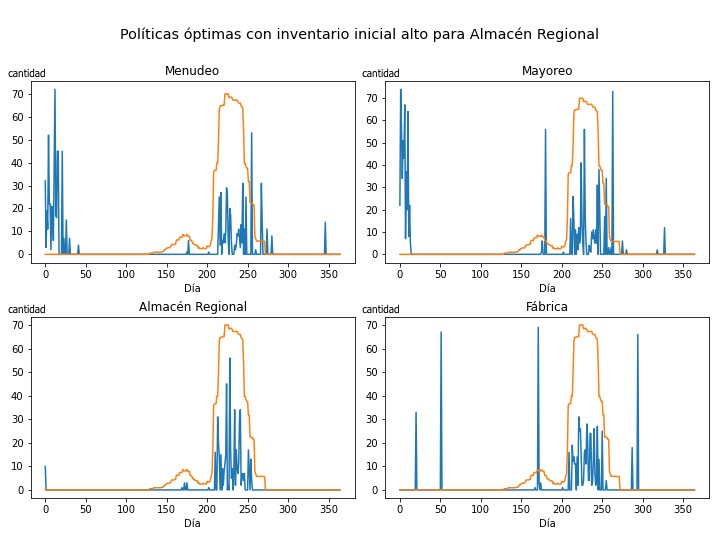
\includegraphics[width=9cm]{tesis_tex/figs/policyiteration_scen_wholesale500.png}
\centering
\end{figure}

\begin{figure}[H]
\caption{Escenario B}
\label{scen_alternative_supply}
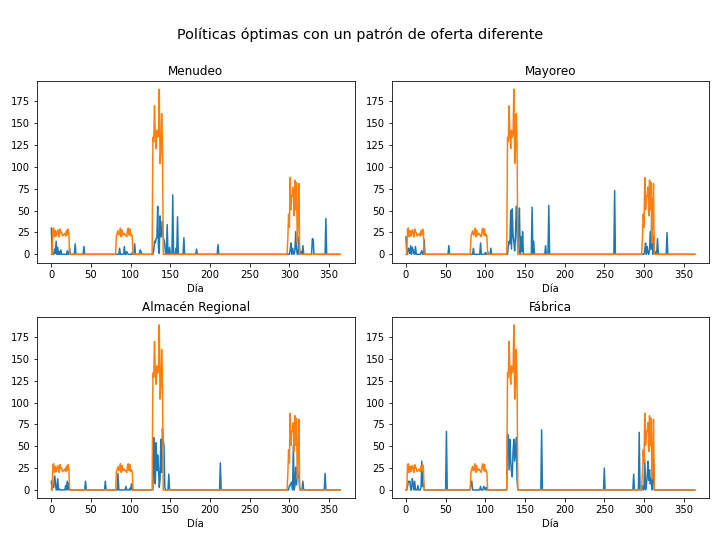
\includegraphics[width=9cm]{tesis_tex/figs/policyiteration_scen_alternativesupply.png}
\centering
\end{figure}
\include{ApendiceB}

%% Incluir la bibliograf'ia. 
\bibliography{Bibliografia}

\end{document}




%%%%%%%%%%%%%%%%%%%%%%%%%% borrar en version final
 % The \cite command functions as follows:
 %   \citet{key} ==>>                Jones et al. (1990)
 %   \citet*{key} ==>>               Jones, Baker, and Smith (1990)
 %   \citep{key} ==>>                (Jones et al., 1990)
 %   \citep*{key} ==>>               (Jones, Baker, and Smith, 1990)
 %   \citep[chap. 2]{key} ==>>       (Jones et al., 1990, chap. 2)
 %   \citep[e.g.][]{key} ==>>        (e.g. Jones et al., 1990)
 %   \citep[e.g.][p. 32]{key} ==>>   (e.g. Jones et al., p. 32)
 %   \citeauthor{key} ==>>           Jones et al.
 %   \citeauthor*{key} ==>>          Jones, Baker, and Smith
 %   \citeyear{key} ==>>             1990
 %---------------------------------------------------------------------
% 
% \begin{center}
%\includegraphics[scale=0.5]{REER1970_Niveles.jpeg}
%\end{center}
% 
% 
% 